%! TEX root = ../main.tex
\documentclass[main]{subfiles}

\begin{document}



\section{主要機能と使用技術}
Teamenverの主な機能は以下の通りである.

\begin{enumerate}
\item 提案表示機能 (2.1節, 図\ref{fig:techstack} Suggestion Function Flow)
\begin{enumerate}
\item メインフレームワークの提案
\item その他ライブラリの提案
\item linter, formatterなどの設定提案
\item ブラウザ上での実行ログの表示
\end{enumerate}
使用技術:Next.js, npm API\cite{npm}, StackOverflow Annual Survey\cite{stackoverflow}

\item コミュニケーション促進機能 (2.2節, 2.3節, 2.4節, 図\ref{fig:techstack} Communication Function Flow)
\begin{enumerate}
\item ユーザの認証・認可
\item リアルタイムチャット
\item ユーザへのロール付与
\item ユーザのオンライン・オフライン表示
\end{enumerate}
使用技術:GraphQL, Hasura Engine
\end{enumerate}
使用した技術の構成を図\ref{fig:techstack}に示す.
\begin{figure}[h]
    \centering
    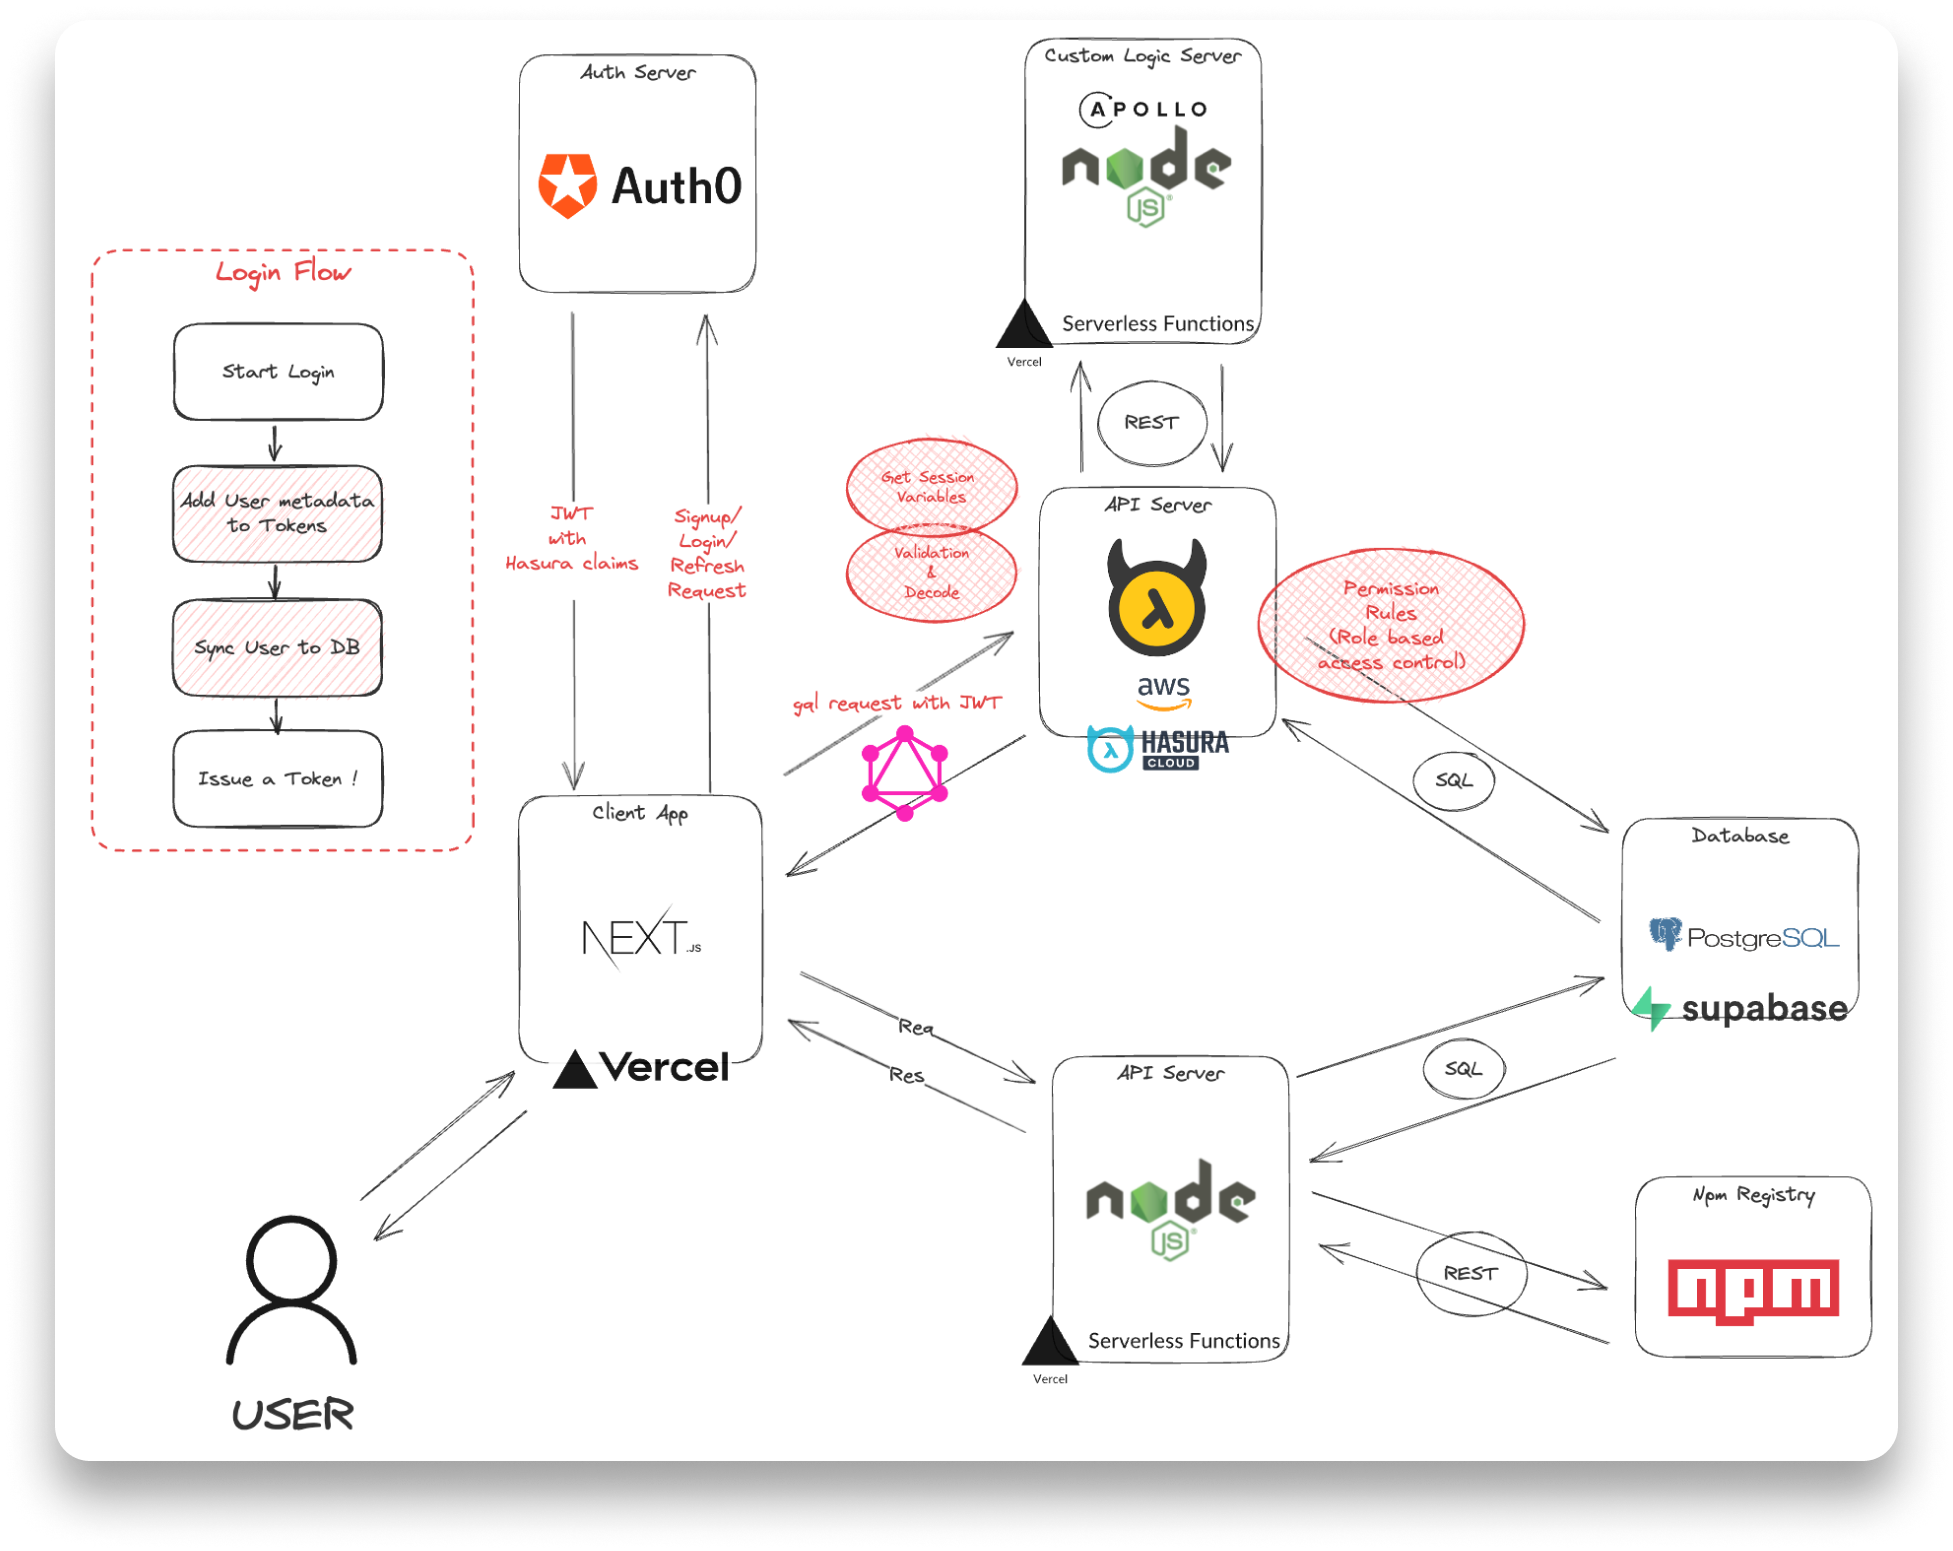
\includegraphics[keepaspectratio,width=0.9\linewidth]{../figures/techstack.pdf}
    \caption{技術構成}
    \label{fig:techstack}
\end{figure}

\end{document}
